\documentclass[]{article}
\usepackage{lmodern}
\usepackage{amssymb,amsmath}
\usepackage{ifxetex,ifluatex}
\usepackage{fixltx2e} % provides \textsubscript
\ifnum 0\ifxetex 1\fi\ifluatex 1\fi=0 % if pdftex
  \usepackage[T1]{fontenc}
  \usepackage[utf8]{inputenc}
\else % if luatex or xelatex
  \ifxetex
    \usepackage{mathspec}
  \else
    \usepackage{fontspec}
  \fi
  \defaultfontfeatures{Ligatures=TeX,Scale=MatchLowercase}
\fi
% use upquote if available, for straight quotes in verbatim environments
\IfFileExists{upquote.sty}{\usepackage{upquote}}{}
% use microtype if available
\IfFileExists{microtype.sty}{%
\usepackage{microtype}
\UseMicrotypeSet[protrusion]{basicmath} % disable protrusion for tt fonts
}{}
\usepackage[margin=1in]{geometry}
\usepackage{hyperref}
\hypersetup{unicode=true,
            pdftitle={MACR Disclosure},
            pdfborder={0 0 0},
            breaklinks=true}
\urlstyle{same}  % don't use monospace font for urls
\usepackage{longtable,booktabs}
\usepackage{graphicx,grffile}
\makeatletter
\def\maxwidth{\ifdim\Gin@nat@width>\linewidth\linewidth\else\Gin@nat@width\fi}
\def\maxheight{\ifdim\Gin@nat@height>\textheight\textheight\else\Gin@nat@height\fi}
\makeatother
% Scale images if necessary, so that they will not overflow the page
% margins by default, and it is still possible to overwrite the defaults
% using explicit options in \includegraphics[width, height, ...]{}
\setkeys{Gin}{width=\maxwidth,height=\maxheight,keepaspectratio}
\IfFileExists{parskip.sty}{%
\usepackage{parskip}
}{% else
\setlength{\parindent}{0pt}
\setlength{\parskip}{6pt plus 2pt minus 1pt}
}
\setlength{\emergencystretch}{3em}  % prevent overfull lines
\providecommand{\tightlist}{%
  \setlength{\itemsep}{0pt}\setlength{\parskip}{0pt}}
\setcounter{secnumdepth}{0}
% Redefines (sub)paragraphs to behave more like sections
\ifx\paragraph\undefined\else
\let\oldparagraph\paragraph
\renewcommand{\paragraph}[1]{\oldparagraph{#1}\mbox{}}
\fi
\ifx\subparagraph\undefined\else
\let\oldsubparagraph\subparagraph
\renewcommand{\subparagraph}[1]{\oldsubparagraph{#1}\mbox{}}
\fi

%%% Use protect on footnotes to avoid problems with footnotes in titles
\let\rmarkdownfootnote\footnote%
\def\footnote{\protect\rmarkdownfootnote}

%%% Change title format to be more compact
\usepackage{titling}

% Create subtitle command for use in maketitle
\newcommand{\subtitle}[1]{
  \posttitle{
    \begin{center}\large#1\end{center}
    }
}

\setlength{\droptitle}{-2em}
  \title{MACR Disclosure}
  \pretitle{\vspace{\droptitle}\centering\huge}
  \posttitle{\par}
  \author{}
  \preauthor{}\postauthor{}
  \date{}
  \predate{}\postdate{}

\usepackage[usenames,dvipsnames,svgnames,table]{xcolor}

\definecolor{lightgray}{gray}{0.975}

\begin{document}
\maketitle

\section{Intro}\label{intro}

This document details the disclosure plan for a \emph{public-use file}
(PUF) based on the California Monthly Arrest and Charge Register (MACR)
database. The PUF is to contain as much information from the MACR as
possible while minimizing the potential for re-identification of
individuals and arrests.

\section{MACR Overview}\label{macr-overview}

The Monthly Arrest and Citation Register reflects monthly arrest reports
from all law enforcement agencies in California since 1980. The reports
are supposed to contain every arrest (and citation until 2005) that an
agency makes of juveniles or adults.

\subsection{Criminal Justice Process}\label{criminal-justice-process}

The MACR contains records of arrests, whether or not those arrests led
to a booking event or eventual prosecution. The following diagram
outlines the possible paths an arrestee might take through the system
and where corresponding data is collected:

\begin{center}
  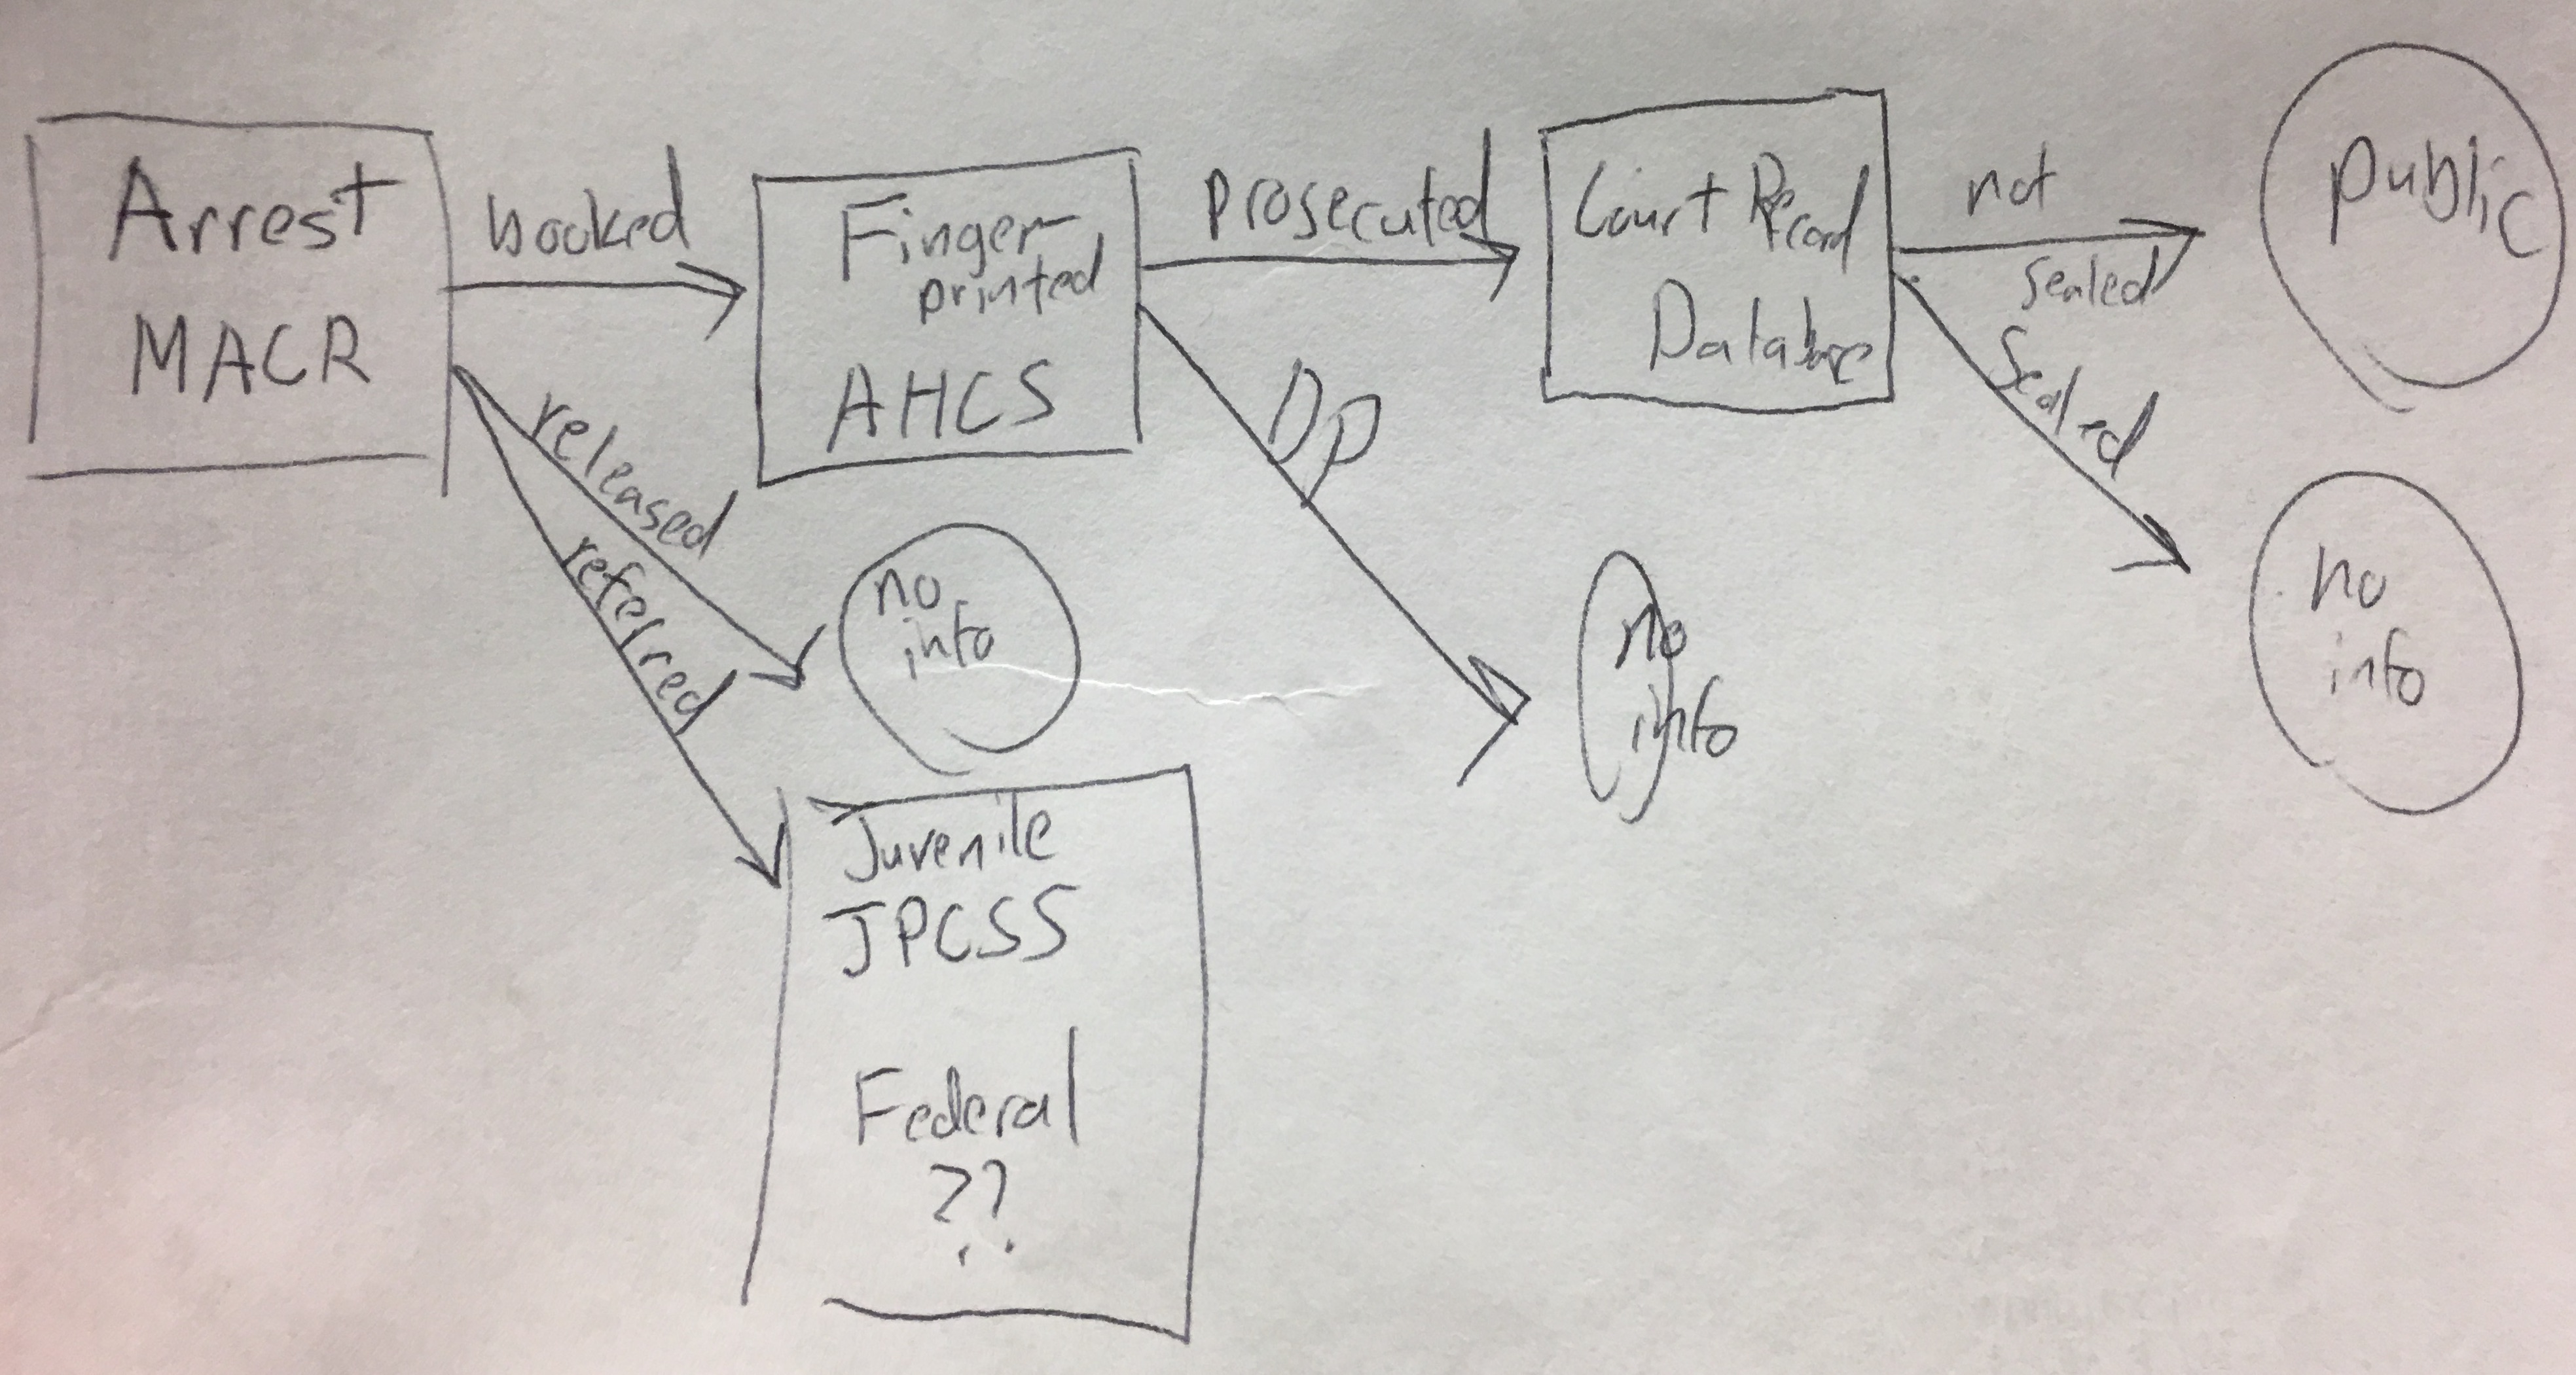
\includegraphics{img/arrestFlowchart.jpg}
\end{center}

For the purposes of disclosure, it is important to note that:

\begin{itemize}
\tightlist
\item
  Many records in the MACR represent instances in which no one was
  convicted of a crime and thus re-identification can lead to personal
  harm (even if many departments facilitate public release of arrest
  data: \href{https://www.localcrimenews.com/welcome/citylist}{example
  arrest publisher})
\item
  There are other sources of data that an attacker could use to
  re-identify an individual in the MACR data, including police
  department feeds and court records.
\item
  A disclosure plan for the MACR needs to account for the possible
  future release of the Offender-Based Transaction Statistics (OBTS) and
  other databases; all datasets to be published need to be collectively
  anonymized.
\end{itemize}

\subsubsection{MACR Records}\label{macr-records}

The MACR contains over 65 million arrests and 21 variables for each,
including values such as the arresting officer's jurisdiction, the
arrest date and BCS code for offense, the age/birth date of the
arrestee, the arrestee's demographics, and the end result of the arrest,
coded as law enforcement `disposition' and the status type of the
arrest. The MACR also contains direct identifiers.

The following is an example of an anonymized, public use file version of
the MACR :

\begin{longtable}[]{@{}llllllll@{}}
\toprule
\begin{minipage}[b]{0.06\columnwidth}\raggedright\strut
year\strut
\end{minipage} & \begin{minipage}[b]{0.07\columnwidth}\raggedright\strut
county\strut
\end{minipage} & \begin{minipage}[b]{0.07\columnwidth}\raggedright\strut
gender\strut
\end{minipage} & \begin{minipage}[b]{0.07\columnwidth}\raggedright\strut
age\strut
\end{minipage} & \begin{minipage}[b]{0.16\columnwidth}\raggedright\strut
race\strut
\end{minipage} & \begin{minipage}[b]{0.08\columnwidth}\raggedright\strut
offense\strut
\end{minipage} & \begin{minipage}[b]{0.14\columnwidth}\raggedright\strut
offense\_level\strut
\end{minipage} & \begin{minipage}[b]{0.14\columnwidth}\raggedright\strut
disposition\strut
\end{minipage}\tabularnewline
\midrule
\endhead
\begin{minipage}[t]{0.06\columnwidth}\raggedright\strut
2015\strut
\end{minipage} & \begin{minipage}[t]{0.07\columnwidth}\raggedright\strut
45\strut
\end{minipage} & \begin{minipage}[t]{0.07\columnwidth}\raggedright\strut
Male\strut
\end{minipage} & \begin{minipage}[t]{0.07\columnwidth}\raggedright\strut
18-24\strut
\end{minipage} & \begin{minipage}[t]{0.16\columnwidth}\raggedright\strut
Asian or Pac Isl\strut
\end{minipage} & \begin{minipage}[t]{0.08\columnwidth}\raggedright\strut
61\strut
\end{minipage} & \begin{minipage}[t]{0.14\columnwidth}\raggedright\strut
status offense\strut
\end{minipage} & \begin{minipage}[t]{0.14\columnwidth}\raggedright\strut
turned ov\ldots{}\strut
\end{minipage}\tabularnewline
\begin{minipage}[t]{0.06\columnwidth}\raggedright\strut
2015\strut
\end{minipage} & \begin{minipage}[t]{0.07\columnwidth}\raggedright\strut
14\strut
\end{minipage} & \begin{minipage}[t]{0.07\columnwidth}\raggedright\strut
Female\strut
\end{minipage} & \begin{minipage}[t]{0.07\columnwidth}\raggedright\strut
18-24\strut
\end{minipage} & \begin{minipage}[t]{0.16\columnwidth}\raggedright\strut
Black\strut
\end{minipage} & \begin{minipage}[t]{0.08\columnwidth}\raggedright\strut
73\strut
\end{minipage} & \begin{minipage}[t]{0.14\columnwidth}\raggedright\strut
misdemeanor\strut
\end{minipage} & \begin{minipage}[t]{0.14\columnwidth}\raggedright\strut
turned ov\ldots{}\strut
\end{minipage}\tabularnewline
\begin{minipage}[t]{0.06\columnwidth}\raggedright\strut
2015\strut
\end{minipage} & \begin{minipage}[t]{0.07\columnwidth}\raggedright\strut
19\strut
\end{minipage} & \begin{minipage}[t]{0.07\columnwidth}\raggedright\strut
Female\strut
\end{minipage} & \begin{minipage}[t]{0.07\columnwidth}\raggedright\strut
18-24\strut
\end{minipage} & \begin{minipage}[t]{0.16\columnwidth}\raggedright\strut
Asian or Pac Isl\strut
\end{minipage} & \begin{minipage}[t]{0.08\columnwidth}\raggedright\strut
17\strut
\end{minipage} & \begin{minipage}[t]{0.14\columnwidth}\raggedright\strut
status offense\strut
\end{minipage} & \begin{minipage}[t]{0.14\columnwidth}\raggedright\strut
complaint\ldots{}\strut
\end{minipage}\tabularnewline
\begin{minipage}[t]{0.06\columnwidth}\raggedright\strut
2015\strut
\end{minipage} & \begin{minipage}[t]{0.07\columnwidth}\raggedright\strut
29\strut
\end{minipage} & \begin{minipage}[t]{0.07\columnwidth}\raggedright\strut
Female\strut
\end{minipage} & \begin{minipage}[t]{0.07\columnwidth}\raggedright\strut
33-44\strut
\end{minipage} & \begin{minipage}[t]{0.16\columnwidth}\raggedright\strut
Other\strut
\end{minipage} & \begin{minipage}[t]{0.08\columnwidth}\raggedright\strut
51\strut
\end{minipage} & \begin{minipage}[t]{0.14\columnwidth}\raggedright\strut
misdemeanor\strut
\end{minipage} & \begin{minipage}[t]{0.14\columnwidth}\raggedright\strut
turned ov\ldots{}\strut
\end{minipage}\tabularnewline
\begin{minipage}[t]{0.06\columnwidth}\raggedright\strut
2015\strut
\end{minipage} & \begin{minipage}[t]{0.07\columnwidth}\raggedright\strut
46\strut
\end{minipage} & \begin{minipage}[t]{0.07\columnwidth}\raggedright\strut
Female\strut
\end{minipage} & \begin{minipage}[t]{0.07\columnwidth}\raggedright\strut
25-32\strut
\end{minipage} & \begin{minipage}[t]{0.16\columnwidth}\raggedright\strut
Hispanic\strut
\end{minipage} & \begin{minipage}[t]{0.08\columnwidth}\raggedright\strut
10\strut
\end{minipage} & \begin{minipage}[t]{0.14\columnwidth}\raggedright\strut
felony\strut
\end{minipage} & \begin{minipage}[t]{0.14\columnwidth}\raggedright\strut
released\strut
\end{minipage}\tabularnewline
\bottomrule
\end{longtable}

County and offense are stored as codes that can be looked up in
accompanying files, such as:

\begin{center}
  \begin{minipage}[t]{0.49\textwidth}
\begin{longtable}[]{@{}ll@{}}
  \toprule
  \begin{minipage}[b]{0.08\columnwidth}\raggedright\strut
  code\strut
\end{minipage} &   \begin{minipage}[b]{0.8\columnwidth}\raggedright\strut
  name\strut
\end{minipage}\tabularnewline
\midrule
\endhead
  \begin{minipage}[t]{0.08\columnwidth}\raggedright\strut
  1\strut
\end{minipage} &   \begin{minipage}[t]{0.8\columnwidth}\raggedright\strut
  Alameda                         \strut
\end{minipage}\tabularnewline
  \begin{minipage}[t]{0.08\columnwidth}\raggedright\strut
  2\strut
\end{minipage} &   \begin{minipage}[t]{0.8\columnwidth}\raggedright\strut
  Alpine/Tuolumne/Calaveras/Amador\strut
\end{minipage}\tabularnewline
  \begin{minipage}[t]{0.08\columnwidth}\raggedright\strut
  3\strut
\end{minipage} &   \begin{minipage}[t]{0.8\columnwidth}\raggedright\strut
  Butte                           \strut
\end{minipage}\tabularnewline
  \begin{minipage}[t]{0.08\columnwidth}\raggedright\strut
  4\strut
\end{minipage} &   \begin{minipage}[t]{0.8\columnwidth}\raggedright\strut
  Colusa/Glenn/Yuba/Sutter/Lake   \strut
\end{minipage}\tabularnewline
  \begin{minipage}[t]{0.08\columnwidth}\raggedright\strut
  5\strut
\end{minipage} &   \begin{minipage}[t]{0.8\columnwidth}\raggedright\strut
  Contra Costa                    \strut
\end{minipage}\tabularnewline
  \bottomrule
\end{longtable}
  \end{minipage}
  \begin{minipage}[t]{0.49\textwidth}
\begin{longtable}[]{@{}ll@{}}
  \toprule
  \begin{minipage}[b]{0.08\columnwidth}\raggedright\strut
  code\strut
\end{minipage} &   \begin{minipage}[b]{0.8\columnwidth}\raggedright\strut
  name\strut
\end{minipage}\tabularnewline
\midrule
\endhead
  \begin{minipage}[t]{0.08\columnwidth}\raggedright\strut
  1\strut
\end{minipage} &   \begin{minipage}[t]{0.8\columnwidth}\raggedright\strut
  Homicide             \strut
\end{minipage}\tabularnewline
  \begin{minipage}[t]{0.08\columnwidth}\raggedright\strut
  2\strut
\end{minipage} &   \begin{minipage}[t]{0.8\columnwidth}\raggedright\strut
  Manslaughter         \strut
\end{minipage}\tabularnewline
  \begin{minipage}[t]{0.08\columnwidth}\raggedright\strut
  3\strut
\end{minipage} &   \begin{minipage}[t]{0.8\columnwidth}\raggedright\strut
  Manslaughter, Vehicle\strut
\end{minipage}\tabularnewline
  \begin{minipage}[t]{0.08\columnwidth}\raggedright\strut
  4\strut
\end{minipage} &   \begin{minipage}[t]{0.8\columnwidth}\raggedright\strut
  Rape                 \strut
\end{minipage}\tabularnewline
  \begin{minipage}[t]{0.08\columnwidth}\raggedright\strut
  5\strut
\end{minipage} &   \begin{minipage}[t]{0.8\columnwidth}\raggedright\strut
  Robbery              \strut
\end{minipage}\tabularnewline
  \bottomrule
\end{longtable}
  \end{minipage}
\end{center}

\section{Disclosure}\label{disclosure}

Disclosure refers to the discovery of potentially harmful information
from the publication of a dataset. Outlining what can be discovered and
how forms the foundation of a plan for disclosure control.

\subsection{Types of Disclosure}\label{types-of-disclosure}

Disclosure can be broken down into \emph{identity disclosure} and
\emph{attribute disclosure}. Identity disclosure refers to learning that
a particular individual is in the dataset (has been arrested) or can be
linked to a particular record (thereby also providing information about
his or her arrest). Attribute disclosure refers to learning something
new about a, possibly unknown individual, such as his or her race.
Whether or not attribute disclosure leads to identity disclosure or is
harmful in and of itself depends on the size of population of people
that match on the attributes. Identity disclosure is also often referred
to as \emph{re-identification}, as it is a partial reversal of the
\emph{de-identification} processes.

\subsection{Potential Harms}\label{potential-harms}

The harms of re-identification depend on the population at risk.

\begin{itemize}
\tightlist
\item
  \emph{juveniles} the purpose of sealing records is to give juveniles a
  clean slate; re-identification would be a significant ethical and
  possibly legal breach
\item
  \emph{victims} in California, victims have a right to privacy and some
  victims can be linked to a perpetrator by the nature of the crime
  (e.g., rape, domestic violence)
\item
  \emph{adults} in general, the harm depends on the severity of the
  crime and the status of the arrest in the criminal justice system

  \begin{itemize}
  \tightlist
  \item
    disclosing an arrest where a person's charge was subsequently
    released can still damage a reputation
  \item
    knowledge of an arrest for a crime that was not fully prosecuted can
    be used for blackmail, or by an illicit background check services in
    an employment scenario
  \end{itemize}
\end{itemize}

Our goal is to avoid giving \emph{new} information to attackers: there
is no privacy risk to individuals where all the information about an
arrest is already public and readily accessible.

\subsection{Variables}\label{variables}

\emph{Direct identifying} variables such as name and date of birth must
always be removed. In the MACR, county, year, and demographic variables
are commonly denoted as \emph{quasi-identifiers} or \emph{key
variables}. If it were possible to match a single instance on these key
variables with, for example, court records, it would be possible to
directly identify an individual. In contrast are so-called
\emph{sensitive variables} that contain information often (but not
always) unique to the MACR, such as the summary offense code, the police
department disposition, and mere existence in the dataset. These roles
are sometimes reversed, specifically when knowledge of an arrest is
already public but knowledge of the specific arrestee is not.

\subsection{External Data}\label{external-data}

External data plays an important role in disclosure control, as it can
be used to match arrests to names or names to crimes. In this section we
only detail external datasets and exclude personal knowledge such as one
might have from witnessing an arrest.

\begin{itemize}
\tightlist
\item
  \emph{court records} At present, online court documentation about
  criminal cases contains limited information with few
  quasi-identifiers. For example, San Diego and Santa Clara counties
  have systems that allow viewing of non-criminal cases, but cripple the
  search system for criminal cases. They show the name and age of the
  defendant, the case number, and the courthouse where the paper copy of
  the case can be found. If CA were ever to consolidate its court
  records statewide, it would probably continue to provide limited
  information about criminal records online. However, a motivated
  attacker can physically obtain some of these records and thus be able
  to match to the MACR.
\item
  \emph{OpenJustice/aggregate arrest data and CJSC reports} Aggregate
  counts of arrests by jurisdiction were previously made available
  online. These have their own disclosure risks but it is important to
  try to minimize the amount of new information that could be gathered
  by comparing the new MACR PUF with previous data. For example, using
  previously published data, an attacker could use counts of arrests by
  demographics to ``un-bin'' the data in the MACR PUF, thereby making it
  easier to identify an individual.
\item
  \emph{OpenJustice Crimes and Clearances data} These data are gathered
  completely separately from the MACR. They try to capture the number of
  crimes that occur in an area and the associated number of individuals
  who are arrested and have a complaint sent to the district attorney's
  office. Because crime counts are based on reports and clearances
  require referral, in general the records in this database do not map
  to records in the MACR. Consequently, OpenJustice Crimes and
  Clearances have limited use in disclosure attempts.
\item
  \emph{crime blotters/local papers} Some papers publish the arrests of
  adults made in local jurisdictions, typically listing the type of
  crime, the age of the arrestee, and often his or her name. This
  information is considered public so that it would not constitute
  disclosure for someone to simply find the associated MACR record if it
  only provides redundant information. However, it is often the case
  that some of the demographic variables (such as race) are excluded
  from these sources.
\item
  \emph{local PD incident reports} Similar to crime blotters, some
  jurisdictions make available summaries of their incident reports. This
  can be used to match the number and types of arrests made.
\item
  \emph{social media} Some arrests have been made public through the use
  of social media, providing partial information about who was arrested,
  what they were arrested for, and/or context about the population
  involved, such as a school, gang, or business.
\item
  \emph{FBI and BJS data} Federal data is much more detailed for crimes
  than arrests. The arrest data is aggregated by 5-6 year periods and
  appears to end in 2012. For arrest data, see:
  \href{https://www.ojjdp.gov/ojstatbb/ezaucr/asp/ucr_display.asp}{Federal
  UCR data}. Once California begins participating in NIBRS, yearly
  city-agency arrest counts will begin to appear here under
  incident-level reporting
  \href{https://ucr.fbi.gov/ucr-publications}{see NIBRS data by state}.
  For states currently on the site, it displays counts of arrests by
  type of crime for the largest cities.
\item
  \emph{US Census} The US Census contains information of the size of
  demographic sub-populations in small counties. When individual
  minorities are incredibly rare in a population, knowledge of a
  matching arrest can imply identity disclosure.
\item
  \emph{background check services/private databases} While the extent of
  these are currently unknown, it should be assumed that some assemblage
  of the previously listed publicly available databases exists.
\end{itemize}

\subsection{Future Data}\label{future-data}

Disclosure control for the MACR needs to take into considerations the
actions of other state agencies as well as plans for future release
within the DoJ.

\subsubsection{CA VoteCal database}\label{ca-votecal-database}

VoteCal, a state-wide voter registration look-up, is not yet a publicly
available tool. Other states that have implemented voter look-up systems
only allow for queries for one voter at a time based on name and county
(and sometimes DoB) - they do not provide lists of voters. None of the
states providing these data included demographic information, such as
gender, race or ethnicity - there would seem to be little reason for
VoteCal to provide demographic information. Race/ethnicity appear in an
optional section of the CA voter registration form. Finally, of the
roughly 39M people living in CA, only \textasciitilde{}17M are
registered to vote.

\subsubsection{Offender-Based Transaction
Statistics}\label{offender-based-transaction-statistics}

The OBTS fields to be released are a super-set of the MACR fields, but
OBTS only contains about 1/4 of the observations of MACR. Approximately
65-75\% of people arrested for a felony end up in the OBTS (e.g., there
were 316K records in 2014). Fields that could be useful to
re-identification attacks or that would help an attacker learn more
about an identified individual:

\begin{itemize}
\tightlist
\item
  demographics and county (same as those in MACR)
\item
  prior record code: no prior, misc prior, one prison commit, two prison
  commits, three prison commits
\item
  arrest offense (5 digit CJIS or penal code) - unlikely to be included
\item
  arrest offense summary code (same as MACR)
\item
  disposition:

  \begin{itemize}
  \tightlist
  \item
    arresting agency reason for release
  \item
    reason for DA decline to prosecute: several reasons, one involves
    victim declining to press charges
  \item
    type of disposition: convict, acquit, not guilty by insanity, etc.
  \item
    sentence: death, prison, jail, fine, etc.
  \item
    convicted offense summary code (same as MACR)
  \end{itemize}
\end{itemize}

\subsubsection{\texorpdfstring{\emph{MACR in Subsequent
Years}}{MACR in Subsequent Years}}\label{macr-in-subsequent-years}

The anonymization plan needs to be able to extend into the future
without requiring changes to past releases. This can be problematic if
randomization is used to add noise to the data, or if new records are
found/old records deleted.

\subsection{Disclosure Methods}\label{disclosure-methods}

In general, there are two types of information that a potential attacker
might seek to discover from the MACR: person \(A\) was arrested for
crime \(X\) or crime \(Y\) was committed by person \(B\). A third type
of identification is simply that person \(C\) was arrested at all. In
this section, we detail the specific process by which a person might go
about discovering this information, forming the basis of a
disclosure-control plan. We distinguish among attacks according the
following types:

\begin{itemize}
\tightlist
\item
  \emph{simple attacks} the basic means by which any attack must proceed
  if disclosure is to take place
\item
  \emph{exclusion attacks} strategies that use external data to derive a
  subset of the MACR in which a simple attack may be more successful
\item
  \emph{disclosure scenarios} detailed descriptions of what an attacker
  might already know, seek to find out, and the ways in which they can
  increase their chances
\end{itemize}

Simple attacks can be prevented by taking limited steps that decrease
the probability of a match or the usefulness of any information
obtained. Exclusion attacks define the different subpopulations in need
of protection. To successfully lead to disclosure, scenarios would
likely proceed through an exclusion attack and employ one or more simple
attacks.

\subsubsection{Simple Attacks}\label{simple-attacks}

\begin{center}
  \renewcommand{\arraystretch}{1.25}
  \rowcolors{2}{lightgray}{}
   \begin{tabular}{p{141.156pt}p{141.156pt}p{141.156pt}}
    \textbf{attack type} & \textbf{disclosure when} & \textbf{remedy} \\ \hline
    match on quasi-identifiers for specific individual                         & quasi-identifiers are unique/rare                                                         & enforce $k$-anonymity for quasi-identifiers by suppressing demographics \\
    match on quasi-identifiers for specific group                              & sensitive values are homogeneous for quasi-identifiers                                    & enforce $l$-diversity for sensitive values by suppressing demographics  \\
    match on partial quasi-identifiers and offense code for unknown individual & quasi-identifiers are homogeneous for offense code                                        & enforce $l$-diversity for quasi-identifiers; aggregate demographics     \\
    match on quasi-identifiers for specific group                              & sensitive values are near homogeneous for quasi-identifiers and all of a similar severity & \color{red}{unknown}                                                   \\
  \end{tabular}
  \renewcommand{\arraystretch}{1.0}
\end{center}

\subsubsection{Exclusion Attacks}\label{exclusion-attacks}

\begin{center}
  \renewcommand{\arraystretch}{1.25}
  \rowcolors{2}{lightgray}{}
   \begin{tabular}{p{117.734pt}p{117.734pt}p{58.867pt}p{117.734pt}}
    \textbf{attack type} & \textbf{disclosure when} & \textbf{risk} & \textbf{remedy} \\ \hline
    exclude prosecuted using court records, perform simple attack on remaining & after exclusion, failure to protect against simple attacks                     & arrested and released                                                             & assume all not released were prosecuted and can be matched; protect released subset when knowledge that arrested is damaging \\
    exclude felony arrests using OBTS, perform simple attack on remaining      & after exclusion, failure to protect against simple attacks                     & arrested for misdemeanor or felony not referred                                   & assume arrests where a complaint was sought for a felony can be matched \emph{from} OBTS; protect complementary subset      \\
    \emph{OBTS attack} use felony arrests in MACR to undo suppression in OBTS & OBTS suppressed information, MACR for felonies did not, perform attack on OBTS & OBTS disclosure                                                                   & assume arrests where a complaint was sought for a felony can be matched \emph{in} OBTS; protect felony arrest subset        \\
    exclusion using court records, OBTS                                        & after exclusion, failure to protect against simple attacks                     & misdemeanor complaint resolved or felony non-prosecution prior to entry into OBTS & none                                                                                                                         \\
  \end{tabular}
  \renewcommand{\arraystretch}{1.0}
\end{center}

\subsubsection{Scenarios}\label{scenarios}

\begin{center}
  \renewcommand{\arraystretch}{1.25}
  \rowcolors{2}{lightgray}{}
   \begin{tabular}{p{86.751pt}p{86.751pt}p{108.439pt}p{130.126pt}}
    \textbf{known quantities} & \textbf{sought quantities} & \textbf{attackers} & \textbf{example} \\ \hline
    quasi-identifiers                               & that arrested              & stalker, blackmailer, background check, employer & minority job interview in small county                     \\
    quasi-identifiers, specific individual arrested & arrest code                & nosy-neighbor, paparazzi, gossips                & saw elderly neighbor get arrested                          \\
    partial quasi-identifiers, offense code         & complete quasi-identifiers & blackmailers, journalists                        & crime blotter mentions age, gender, and crime but not race \\
    offense code, disposition                       & quasi-identifiers          & journalist, blackmailer / fisher                 & unusual crime committed by minority                        \\
    offense code, arrest circumstances              & quasi-identifiers          & coworkers, gossips                               & tweet mentions crime by an employee at a business          \\
    specific individual, offense code               & disposition                & journalist, employer                             & local crime blotter mentions name and crime                \\
  \end{tabular}
  \renewcommand{\arraystretch}{1.0}
\end{center}

\subsection{Disclosure Scenario
Summary}\label{disclosure-scenario-summary}

\begin{itemize}
\tightlist
\item
  Knowing only quasi-identifiers with the aim of obtaining information
  about the arrest code or disposition can only succeed when the set of
  matches are singular or homogeneous. Addressing \(k\)-anonymity and
  \(l\)-diversity (detailed below) through suppression and aggregation
  should be sufficient.
\item
  When the arrest code is known and quasi-identifiers are the goal, it
  is important that there be diversity in the keys that match each
  arrest code. This depends on how many quasi-identifiers are already
  known and the rarity of the arrest code. For a really rare code (e.g.,
  bookmaking) the demographics across the entire state may be sufficient
  to discover the race and age of the arrestees, leading to
  identification. Anonymity can be achieved by either suppressing the
  offense codes, aggregating offense codes, or by selectively
  suppressing demographics for individuals who have committed rare
  crimes.
\item
  External knowledge from court records imply that every record that led
  to successful prosecution needs to be assumed to be public and can be
  used in an exclusion attack. We run a separate anonymization process
  for those who were arrested and then had their charge ``released''
  (disposition) and then anonymize them again as part of the entire MACR
  PUF file.
\item
  External knowledge from a future OBTS publication has similar
  consequences, but the anonymization must go both ways.
\item
  Discovery of the disposition field seems to be of low risk, with the
  primary consequences of disclosure reflecting on the practices of the
  police department and district attorney's office.
\end{itemize}

\section{Anonymization Plan}\label{anonymization-plan}

\subsection{Preliminary Steps}\label{preliminary-steps}

Anonymization at this stage consists largely of aggregation into coarser
categories based on substantive knowledge. This serves to decrease the
risks of identification, but also naturally models steps that a
researcher might otherwise take to create explanatory models.

\begin{itemize}
\tightlist
\item
  remove direct identifiers
\item
  remove juveniles
\item
  discretize age into four categories: 18-24, 25-32, 33-44, 45+
\item
  combine smaller racial or ethnic groups to leave: White, Black,
  Hispanic, Asian or Pacific Islander, Other
\item
  aggregate jurisdictions into counties
\item
  combine small counties into geographic entities
\end{itemize}

\subsection{Routine Protection}\label{routine-protection}

We have made mention of two forms of risk analysis, \(k\)-anonymity and
\(l\)-diversity. The first refers to the number of records that share a
complete set of quasi-identifiers while the second refers to the number
of different sensitive values that share a complete set of
quasi-identifiers. If either is small, then there is a substantial risk
of disclosure. For each record in the MACR and for any chosen variables,
these values can be computed and an anonymizing action taken. Based on
the above, we compute:

\begin{itemize}
\tightlist
\item
  \(k\) anonymity for the quasi-identifiers of year, county, gender,
  race, and age
\item
  \(l\) diversity given the same quasi-identifiers and the sensitive
  value of offense code
\item
  \(l\) diversity for the quasi-identifier of offense code and the
  sensitive value of the combination of year, gender, race, and age
\end{itemize}

If, for any arrest, one of these is below 3 then the county variable for
that entry is suppressed.

\subsection{Population Protection}\label{population-protection}

Because of exclusion attacks, some subsets of the data are at risk and
require the above steps to be applied just to them. These are:

\begin{itemize}
\tightlist
\item
  arrests with a disposition of released and an offense code where being
  arrested and then released carries an implication of guilt
\item
  arrests with a disposition of complaint sought and offense level of
  felony
\item
  arrests with the complementary set of conditions, that is a
  disposition that is not complaint sought or an offense level that is
  not felony
\end{itemize}

Finally, the population as a whole was given the same treatment.


\end{document}
